\chapter{Methods \label{chap:methods}}
\graphicspath{{chapters/methods/}}
This chapter introduces the base algorithms from which the task-based algorithms in the next chapters are derived.
The dense linear algebra algorithms will be presented then the sparse linear algebra and finally, the Kirchhoff seismic pre-stack depth migration.

\section{Dense Linear Algebra}

This section focus on the dense linear methods we consider as benchmark to experiment on the programming models.
We introduce the LU factorization and three methods to solve a linear system namely the Gaussian elimination, the Gauss-Jordan elimination and the LU factorization.
We introduce the regular point to point methods as well as the block based methods.


The LU factorization and the solution of linear systems are two very useful dense linear algebra operations.
They are used as base for more complex operations like linear solvers.
For instance, the LU factorization to solve a linear system is used a benchmark which is called LINPACK \cite{Parle1981} \cite{DonLP2003} for the TOP 500 which ranks the performances of the supercomputers.
The LU factorization is also used to invert a matrix in LAPACK \cite{ABBBD1999} and its distributed counterpart ScaLAPACK \cite{ChDPW1992} \cite{BCCDD1996}.

These implementations are considered as using block algorithms.
However, the term "block" as several meanings in the literature as shown in \cite{DemHS1995}.
According to \cite{DemHS1995}, the algorithms used in LINPACK, LAPACK and ScaLAPACK as explained in \cite{CDOPW1996} are better termed as \textit{partitioned algorithms} which "is a scalar algorithm in which the operations have been grouped and reordered as matrix operations" whereas block algorithms are "a generalization of a scalar algorithm in which the basic scalar operations become matrix operations ($\alpha + \beta, \alpha\beta, \alpha / \beta$ become $A+B, AB, AB^{-1}$)"

In this section, we are interested in the block algorithms referring to a generalization of the scalar algorithms.
Therefore, this explain why our algorithms are different from ScaLAPACK's.


% eigenvalues, eigenvectors ?


\subsection{Block-Based LU factorization to Solve Linear Systems}

The block LU factorization problem is introduced in \cite{DemHS1995} \cite{GoluL1983} \cite{BuncR1976}.
It consists in finding $L$ and $U$ such as $A=L\cdot U$ where $L$ is a block lower triangular matrix of size $p \times p$ with identity on the diagonal and $U$ is a block upper triangular matrix of size $p\times p$ (see Equation \ref{eq:a_eq_lu}).
However, in general, the $U_{ii}$ blocks are not triangular.
They may be complete matrices.

\begin{equation}
	\label{eq:a_eq_lu}
	A =
	\begin{bmatrix*}[l]
	A_{1,1} & A_{1,2} & A_{1,3}\\
	A_{2,1} & A_{2,2} & A_{2,3}\\
	A_{3,1} & A_{3,2} & A_{3,3}
	\end{bmatrix*}
	=
	\begin{bmatrix*}[l]
	I       &         &\\
	L_{2,1} & I       &\\
	L_{3,1} & L_{3,2} & I
	\end{bmatrix*}
	\begin{bmatrix*}[l]
	U_{1,1} & U_{1,2} & U_{1,3}\\
	        & U_{2,2} & U_{2,3}\\
	        &         & U_{3,3}
	\end{bmatrix*}
	=
	LU
\end{equation}


We consider LU factorization $A=LU \in \mathbb{R}^{n \times n}$ partitioned as follow where the diagonal blocks are square but are not necessarily of the same dimension.
If $A_{11}$ is nonsingular, we can write
\begin{equation}
	\label{eq:a_eq_lu_schur}
	A =
	\begin{bmatrix*}[l]
	A_{1,1} & A_{1,2}\\
	A_{2,1} & A_{2,2}
	\end{bmatrix*}
	=
	\begin{bmatrix*}[l]
	I       & \\
	L_{2,1} & I
	\end{bmatrix*}
	\begin{bmatrix*}[l]
	A_{1,1} & A_{1,2}\\
	        & S
	\end{bmatrix*}
\end{equation}

Equation \ref{eq:a_eq_lu_schur} describes a step of a recursive algorithm to compute a block LU factorization where $S = A_{2,2} - A_{2,1}A_{1,1}^{-1}A_{1,2}$ is a Schur complement of A.
If we partition S and its $(1,1)$ block is nonsingular, we can factorize S in a similar manner.
This process can be repeated until a complete LU factorization is obtained.
Algorithm \ref{alg:reclufact_block} shows this process.


\begin{algorithm}[h]
	\DontPrintSemicolon
	%\SetAlgoVlined
	\caption{Recursive Block (Generalized) LU Factorization\label{alg:reclufact_block}}
	Partition the matrix A : $U_{1,1} = A_{1,1},U_{1,2} = A_{1,2}$\;
	Solve $L_{2,1}A_{1,1} = A_{2,1}$ for $L_{2,1}$\;
	$S = A_{2,2} - A_{2,1}A_{1,1}^{-1}A_{1,2}$\;
	Repeat this process on S
\end{algorithm}

Algorithm \ref{alg:lufact_block} introduces a non-recursive algorithm for the block LU factorization.

\begin{algorithm}[h]
	\DontPrintSemicolon
	%\SetAlgoVlined
	\caption{Block (Generalized) LU Factorization\label{alg:lufact_block}}
	\For{k \KwFrom 0 \KwTo p-2}{
		(1) $\displaystyle Inv^{(k)} = [A_{k,k}^{(k)}]^{-1}$ \;
		\For{i \KwFrom k+1 \KwTo p-1}{
			(2) $\displaystyle A_{i,k}^{(k+1)} = A_{i,k}^{(k)} \cdot Inv^{(k)}$ \;
			\For{j \KwFrom k+1 \KwTo p-1}{
				(3) $A_{i,j}^{(k+1)} = A_{i,j}^{(k)} - A_{i,k}^{(k+1)} \cdot A_{k,j}^{(k)}$ \;
			}
		}
	}
\end{algorithm}

The goal here is to solve the linear system $Ax = b$ by replacing $A$ by its LU factorization.
Therefore, the problem becomes solving the system $LUx=b$.
There is two triangular linear systems to solve : $Ly=b$ then $Ux=y$.
Algorithm \ref{alg:lufact_sls} solves the linear system $Ax = b$ to obtain $x$ given the LU factorization of $A$ stored in one matrix and $b$.

\begin{algorithm}[h]
	\DontPrintSemicolon
	%\SetAlgoVlined
	\caption{Solution of a linear system with a block-based LU factorization\label{alg:lufact_sls}}
	\For{i \KwFrom 0 \KwTo p-2}{
		\For{j \KwFrom i+1 \KwTo p}{
			(5) $b_j^{(i+1)} = b_j^{(i)} - A_{j,i}^{(i+1)} \cdot b_i^{(p)}$ \;
		}
	}
	\;
	\For{k \KwFrom p-1 \KwTo 0 \KwStep -1}{
		(6) solve $b_{k}^{(p)} = A_{k,k}^{(k)} \cdot b_k^{(p-1)}$ \;
		\For{i \KwFrom 1 \KwTo k-1}{
			(7) $b_i^{(p-k+i)} = b_i^{(p-k+i-1)} - A_{i,k}^{(i)} \cdot b_k^{(p)}$ \;
		}
	}
\end{algorithm}

%\cite{GeisR1988}
%\cite{HendW1994}
%\cite{DonGW1994}
%\cite{Straz1995}

The block LU algorithm can also be obtained from the scalar algorithm since the it can be generalized by changing from scalar to matrices and using the appropriate operations.
The scalar algorithm with pivot for the LU factorization can be found in \cite{BissV1988} \cite{Velde1990}.
However, there is no pivoting in the block algorithm although pivoting may be used to increase the stability during the inversion of the diagonal blocks.
Algorithm \ref{alg:lufact_scalar} is a scalar version without pivot of the LU factorization \cite{GoluL1983}.

\begin{algorithm}[h]
	\DontPrintSemicolon
	%\SetAlgoVlined
	\caption{Scalar LU Factorization\label{alg:lufact_scalar}}
	\For{k \KwFrom 0 \KwTo p-2}{
		\For{i \KwFrom k+1 \KwTo p-1}{
			(1) $\displaystyle a_{i,k}^{(k+1)} = a_{i,k}^{(k)} / a^{(k)}$ \;
			\For{j \KwFrom k+1 \KwTo p-1}{
				(2) $a_{i,j}^{(k+1)} = a_{i,j}^{(k)} - a_{i,k}^{(k+1)} \cdot a_{k,j}^{(k)}$ \;
			}
		}
	}
\end{algorithm}

The LU factorization is based on the Gaussian elimination which will can also be used to solve linear systems.

\subsection{Block-Based Gaussian Elimination to Solve Linear Systems}

The scalar Gaussian elimination algorithm with pivoting is discussed in \cite{Saad1986} and \cite{GeorC1987}.
The pivoting increase the numerical stability of the operations.
However, in the case of block algorithms with a generalization of the scalar operations into a matrix operation, pivoting the rows of sub-matrices means that we need to find a way to determine which matrix could be used as a pivot.
Moreover, the increase in numerical stability of such method is unknown.
This topic is not discussed in this work.
Furthermore, the algorithm which is used as base for generalization in the LU factorization does not use pivoting on the sub-matrices.
Although, pivoting may be used to improve the numerical stability in the inversion of the sub-matrices.
Algorithm \ref{alg:bg_el_scalar} introduces a scalar Gaussian elimination without pivoting \cite{GoluL1983} which will be generalized into a block algorithm in Algorithm \ref{alg:bg_el_block}.
These two algorithms are used to solve a linear system and include the back substitution which allow to compute the solution of the linear system.


\begin{algorithm}[h]
	\DontPrintSemicolon
	\caption{Scalar Gaussian elimination and back substitution \label{alg:bg_el_scalar}}
	%\scriptsize
	\For{k \KwFrom 0 \KwTo p-2}{
		(1) $b_k^{(k+1)} = b_k^{(k)} / a_{k,k}^{(k)}$ \;
		\For{j \KwFrom k+1 \KwTo p-1}{
			(2) $ a_{k,j}^{(k+1)} = a_{k,j}^{(k)} / a_{k,k}^{(k)}$ \;
		}
		\For{i \KwFrom k+1 \KwTo p-1}{
			(3) $b_i^{(k+1)} = b_i^{(k)} - a_{i,k}^{(k)} \cdot b_k^{(k+1)}$ \;
			\For{j \KwFrom k+1 \KwTo p-1}{
				(4) $a_{i,j}^{(k+1)} = a_{i,j}^{(k)} - a_{i,k}^{(k)} \cdot a_{k,j}^{(k+1)}$ \;
			}
		}
	}

	(5) $b_{p-1}^{(p)} = b_{p-1}^{(p-1)} / a_{p-1,p-1}^{(p-1)} $ \;

	\For{k \KwFrom 1 \KwTo p-1 }{
		\For{i \KwFrom 0 \KwTo p-k-1 }{
			(6) $b_i^{(k+i+1)} = b_i^{(k+i)} - a_{i,p-k}^{(i+1)} \cdot b_{p-k}^{(p)}$ \;
		}
	}
\end{algorithm}

The Gaussian elimination has a similar number of block operations as the block LU factorization but the critical path of the graph of operations is significantly shorter than the one in the block LU factorization since there is only one solution of a triangular system after the operations on the matrix whereas there is two in the block LU factorization.
This means that the block LU factorization and the block Gaussian elimination have different performances.

\begin{algorithm}[h]
	\DontPrintSemicolon
	\caption{Block (Generalized) Gaussian elimination and back substitution \label{alg:bg_el_block}}
	%\scriptsize
	\For{k \KwFrom 0 \KwTo p-2}{
		(1) $\displaystyle Inv^{(k)} = [A_{k,k}^{(k)}]^{-1}$ \;
		(2) $b_k^{(k+1)} = Inv^{(k)} \cdot b_k^{(k)}$ \;
		\For{j \KwFrom k+1 \KwTo p-1}{
			(3) $\displaystyle A_{k,j}^{(k+1)} = Inv^{(k)} \cdot A_{k,j}^{(k)} $ \;
		}
		\For{i \KwFrom k+1 \KwTo p-1}{
			(4) $b_i^{(k+1)} = b_i^{(k)} - A_{i,k}^{(k)} \cdot b_k^{(k+1)}$ \;
			\For{j \KwFrom k+1 \KwTo p-1}{
				(5) $A_{i,j}^{(k+1)} = A_{i,j}^{(k)} - A_{i,k}^{(k)} \cdot A_{k,j}^{(k+1)}$ \;
			}
		}
	}

	(6) $b_{p-1}^{(p)} = Inv^{(p-1)} \cdot b_{p-1}^{(p-1)}$ \;

	\For{k \KwFrom 1 \KwTo p-1 }{
		\For{i \KwFrom 0 \KwTo p-k-1 }{
			(7) $b_i^{(k+i+1)} = b_i^{(k+i)} - A_{i,p-k}^{(i+1)} \cdot b_{p-k}^{(p)}$ \;
		}
	}
\end{algorithm}



\subsection{Block-Based Gauss-Jordan Elimination to Solve Linear Systems}

The Gauss-Jordan elimination \cite{Petit1989} \cite{Attaw2012} is similar to the Gaussian elimination except that the computations made under the diagonal are also performed above it while directly outputting the solution of the linear system.
Algorithm \ref{alg:bgj_scalar} is a scalar Gauss-Jordan elimination algorithm without pivoting \cite{Attaw2012}.
It is indeed very similar to Algorithm \ref{alg:bg_el_scalar} which is the Gaussian elimination with the mentioned modifications.
This algorithm is also converted into a generalized block Gauss-Jordan elimination \cite{MelTP1999} in Algorithm \ref{alg:bgj_block}.

\begin{algorithm}[h]
	\DontPrintSemicolon
	\caption{Scalar Gauss-Jordan elimination to solve a linear system \label{alg:bgj_scalar} }
	\For{k \KwFrom 0 \KwTo p-1}{
		(1) $b_k^{(k+1)} =  b_k^{(k)} / a_{k,k}^{(k)}$ \;
		\For{j \KwFrom k+1 \KwTo p-1}{
			(2) $\displaystyle a_{k,j}^{(k+1)} = a_{k,j}^{(k)} / a_{k,k}^{(k)}$ \;
			\For{i \KwFrom 0 \KwTo p-1}{
				\If{k $\neq$ i}{
					(3) $a_{i,j}^{(k+1)} = a_{i,j}^{(k)} - a_{i,k}^{(k)} \cdot a_{k,j}^{(k+1)}$ \;
				}
			}
		}
		\For{i \KwFrom 0 \KwTo p-1}{
			\If{k $\neq$ i}{
				(4) $b_i^{(k+1)} = b_i^{(k+1)} - a_{i,k}^{(k)} \cdot b_k^{(k+1)}$ \;
			}
		}
	}
\end{algorithm}

The Gauss-Jordan elimination has more block operations than the block Gaussian elimination and the block LU factorization but the critical path of the block operations is even shorter than the Gaussian Elimination since there is no solution of triangular systems.
Although, there is more block operations than the two other block algorithms but the critical path is shorter.
This means that there is more block operations that can be performed in parallel during the elimination.
This also means that this algorithm may be able to run faster than the two other block algorithms on a parallel machine.

\begin{algorithm}[h]
	\DontPrintSemicolon
	\caption{Block (Generalized) Gauss-Jordan elimination to solve a linear system \label{alg:bgj_block} }
	\For{k \KwFrom 0 \KwTo p-1}{
		(1) $\displaystyle Inv^{(k)} = [A_{k,k}^{(k)}]^{-1}$ \;
		(2) $b_k^{(k+1)} = Inv^{(k)} \cdot b_k^{(k)}$ \;
		\For{j \KwFrom k+1 \KwTo p-1}{
			(3) $\displaystyle A_{k,j}^{(k+1)} = Inv^{(k)} \cdot A_{k,j}^{(k)} $ \;
			\For{i \KwFrom 0 \KwTo p-1}{
				\If{k $\neq$ i}{
					(4) $A_{i,j}^{(k+1)} = A_{i,j}^{(k)} - A_{i,k}^{(k)} \cdot A_{k,j}^{(k+1)}$ \;
				}
			}
		}
		\For{i \KwFrom 0 \KwTo p-1}{
			\If{k $\neq$ i}{
				(5) $b_i^{(k+1)} = b_i^{(k+1)} - A_{i,k}^{(k)} \cdot b_k^{(k+1)}$ \;
			}
		}
	}
\end{algorithm}

In this section, we introduced the different meaning of block algorithm : the algorithms where the scalar operations are generalized into matrix operations or algorithms where the operations are reorganized in order to perform matrix operations (usually matrix product) on subset of the initial matrix.
Moreover, we introduced the scalar and block algorithms for the LU factorization, the Gaussian elimination and the Gauss-Jordan elimination.
Dense linear system solution is widely used in solvers for simulations so it is important to create robust and efficient library providing these operation since it will save time and computational resources.
Simulations can also create sparse matrices to represent the simulated environment.
In this case, direct method to solve linear systems based on the Gaussian elimination are not suitable since the factorization modify the rows of the matrices and may introduce new values at places where there is zeros in the sparse matrix.
Iterative methods do not modify the input matrix and are used to deal with the sparse matrices.
Most of these iterative methods are based on the sparse matrix vector product which will be discussed in the next section.


\section{Sparse Linear Algebra}

Discretization of partial differential equation in numerical simulations often leads to the creation of a linear system which has to be resolved in order to solve the equation.
The linear system is most of the time stored as a matrix.
When the matrix is dense, direct methods can be used to solve the linear system as seen in the previous section.
However, the discretization of the partial differential equation can produce linear system where the matrix contains a lot of zero.
In this case, the matrix is considered sparse and is stored using sparse storage formats.
Some of the most commonly used sparse matrix storage formats are discussed in this section.
Moreover, the direct methods are not suitable to solve sparse linear systems since it introduce new values in the matrix during the Gaussian elimination.
Modifying a sparse matrix is difficult since depending on the storage format the row or the columns are compressed (the zero are removed from the arrays) so inserting new values means creating a new array and copying the previous values while adding the new one.
Therefore, avoiding insertion in sparse matrix improves the performances greatly since the copy is very expensive.
This leads to the use of iterative sparse methods to solve linear systems.
These methods heavily rely on sparse matrix vector product.
There is also several other methods that rely on sparse matrix vector product like the conjugate gradient, the Lanczos methods, the Krylov subspaces \cite{Saad1989} \cite{Saad2003}, Page Rank \cite{RidiS2002} and an essential part of many graph kernels \cite{KepnG2011}.
Even hardware prototypes \cite{SoGLK2016} have been designed to improve the graph computational throughput compared to conventional hardware.

In this section, we will focus on the different sparse matrix storage and their corresponding matrix vector product implementation.

\subsection{Sparse Matrix Storage and Sparse Matrix-Vector Multiplication}

Sparse matrix format are used to store and process sparse matrices in a wide range of domains and libraries.
SPARSKIT \cite{Saad1990} is a library which provides routines to convert matrices in one sparse format to another one.
It also provides a set of routines to make operation on sparse matrices like matrix vector product, eigenvalues computations and linear system solving.
The following sections will describe several widely used sparse matrices formats and give the algorithm to compute a matrix vector product with those formats.

\subsubsection{Dense}
Dense is the classical and most straightforward format used to store matrices.
It is usually used for matrices with a few number of null values.
In the case of sparse matrices, it is not efficient since it stores a large amount of unused values (the zeros).
Those zeros will also be part of computations while making operations on the matrix.
Therefore, storing the sparse matrices into a more adapted format will reduce memory footprint and save operations on zeros.
Figure \ref{fig:methods:dense_ex} shows a $5 \times 5$ sparse matrix stored as a dense matrix.

\begin{figure}
\centering
\begin{tabular}{|ccccc|}
\hline
1 & 2 & 0 & 0 & 3 \\
0 & 0 & 4 & 0 & 0 \\
0 & 5 & 0 & 0 & 0 \\
0 & 6 & 0 & 7 & 0 \\
8 & 0 & 9 & 0 & 10 \\
\hline
\end{tabular}
\caption{Sparse matrix stored in dense format \label{fig:methods:dense_ex}}
\end{figure}

\begin{algorithm}[h]
	\DontPrintSemicolon
	\caption{Matrix vector multiplication - dense\label{fig:methods:dense_algo}}
	%\scriptsize
	\For{i = 1, $N_{row}$}{
		y[i] = 0.0 \;
		\For{j = 1, $N_{col}$}{
			$y[i] \pluseq val[i,j] \times x[i]$ \;
		}
	}
\end{algorithm}

\subsubsection{Coordinates - COO}
COO are the first letters of the word coordinates which summarize how the sparse matrices will be stored in this format.
It uses two two vectors to store the two dimensional coordinates of the value in the matrix and another vector which contains the values.
It is a key-value storage type.
The key is the coordinates of the value in the matrix.

The COO format is used in TensorFlow to store sparse matrices into tensors.
%used in MaP Reduce

The COO format has several useful properties.
The values can be easily split and distributed by dividing the three vectors while keeping the coordinates-values pairs.
It is also a format that allows easy construction of matrices since the addition of new values is easy.
Indeed, they can easily be added at the end of the three vectors.
The transposition is fast.
Only, the row and the column vectors have to be exchanged.

Figure \ref{fig:methods:coo_ex} shows an example of the storage of the example matrix in COO format.

\begin{figure}
\centering
row
\bigskip
\begin{tabular}{|cccccccccc|}
\hline
0 & 0 & 0 & 1 & 2 & 3 & 3 & 4 & 4 & 4  \\
\hline
\end{tabular}

col
\bigskip
\begin{tabular}{|cccccccccc|}
\hline
0 & 1 & 4 & 2 & 1 & 1 & 3 & 0 & 2 & 4 \\
\hline
\end{tabular}

val
\bigskip
\begin{tabular}{|cccccccccc|}
\hline
1 & 2 & 3 & 4 & 5 & 6 & 7 & 8 & 9 & 10 \\
\hline
\end{tabular}
\caption{Sparse matrix stored in COO format \label{fig:methods:coo_ex}}
\end{figure}

\begin{algorithm}[h]
	\DontPrintSemicolon
	\caption{Matrix vector multiplication - COO\label{fig:methods:coo_algo}}
	%\scriptsize
	\For{i = 1, $N_{row}$}{
		y[i] = 0.0 \;
	}
	\For{i = 1, NNZ}{
		$y[row[i]] \pluseq val[i] \times x[col[i]]$ \;
	}
\end{algorithm}

\subsubsection{Compressed Sparse Row - CSR}
The Compressed Sparse Row format (CSR) \cite{HacBG1971} \cite{Gusta1972} is a derivation of the COO format where the vector containing the index of the rows is compressed.
The array giving the row index of the value at the same position in the array of values is replaced by an array which gives the position of the beginning of each row in the column array.
In COO, the row array has NNZ values (the number of non zero values) whereas there is only $N+1$ values (N is the dimension of the matrix) where N is smaller than NNZ.
Therefore, it saves space in memory.

However, inserting new values in a matrix stored in the CSR format implies to move the values in the column and values arrays after the inserted value.

Figure \ref{fig:methods:csr_ex} shows an example of the storage of the example matrix in CSR format.

\begin{figure}
\centering
idx
\bigskip
\begin{tabular}{|cccccc|}
\hline
0 & 3 & 4 & 5 & 7 & 10 \\
\hline
\end{tabular}

col
\bigskip
\begin{tabular}{|cccccccccc|}
\hline
0 & 1 & 4 & 2 & 1 & 1 & 3 & 0 & 2 & 4 \\
\hline
\end{tabular}

val
\bigskip
\begin{tabular}{|cccccccccc|}
\hline
1 & 2 & 3 & 4 & 5 & 6 & 7 & 8 & 9 & 10 \\
\hline
\end{tabular}
\caption{Sparse matrix stored in CSR format \label{fig:methods:csr_ex}}
\end{figure}


\begin{algorithm}[h]
	\DontPrintSemicolon
	\caption{Matrix vector multiplication - CSR\label{fig:methods:csr_algo}}
	%\scriptsize
	\For{i = 1, $N_{row}$}{
		y[i] = 0.0 \;
		\For{j = idx[i], idx[i+1]}{
			$y[i] \pluseq val[j] \times x[col[j]]$ \;
		}
	}
\end{algorithm}


\subsubsection{Diagonal - DIA}
The diagonal format (DIA) is very useful in the case of matrices which have a pattern where the non-zero are located in a small amount of diagonals.
It is composed of two arrays : a one dimensional array which represents the offsets from the diagonal of the values in the associated column and a two dimensional array with the values in each row in the column associated to their offset from the diagonal.
The values array needs to be padded with zeros where there no values from the initial matrix in order to be used in the algorithms.
This format is designed for matrices where diagonals are very populated since it needs a column in the values array for each diagonal where there is values.

Figure \ref{fig:methods:dia_ex} shows an example of the storage of the example matrix in diagonal format.
However, this example is not adapted to the diagonal storage format since it leaves a lot of padding values in the values matrices.
For this format, a matrix where is non-zero values are located on the same diagonals is more interesting.

\begin{figure}
\centering
\begin{tabular}{c|cccccc|}
	\cline{2-7}
	        offset          & -4 & -2 & -1 & 0  & 1 & 4 \\ \cline{2-7}
	\multirow{5}{*}{values} & 0  & 0  & 0  & 1  & 2 & 3 \\
	                        & 0  & 0  & 0  & 0  & 4 & 0 \\
	                        & 0  & 0  & 5  & 0  & 0 & 0 \\
	                        & 0  & 6  & 0  & 7  & 0 & 0 \\
	                        & 8  & 9  & 0  & 10 & 0 & 0 \\ \cline{2-7}
\end{tabular}
\caption{Sparse matrix stored in diagonal format \label{fig:methods:dia_ex}}
\end{figure}

\begin{algorithm}[h]
	\DontPrintSemicolon
	\caption{Matrix vector multiplication - DIA\label{fig:methods:dia_algo}}
	%\scriptsize
	\For{i = 1, $N_{row}$}{
		y[i] = 0.0 \:
		\For{j = 1, $n\_diag$}{
			$y[i] \pluseq  values[i,j] \times x[i+offset(j)]$ \;
		}
	}
\end{algorithm}


\subsubsection{Ellpack-Itpack - ELL}
The Ellpack-Itpack format (ELL) is a generalization of the diagonal format.
It uses two arrays with two dimensions to store the position of the values in the columns and the values.
Each row of those arrays store the values in the rows of the original matrix without zeros and the column array store the column index of the value in the original matrix.
The values array needs to be padded with zeros where there no values from the initial matrix in order to be used in the algorithms.

Figure \ref{fig:methods:ell_ex} shows an example of the storage of the example matrix in Ellpack-Itpack format.


\begin{figure}
\centering
\begin{tabular}{c|ccc|}
	\cline{2-4}
	\multirow{5}{*}{values}  & 1 & 2 & 3  \\
	                         & 4 & 0 & 0  \\
	                         & 5 & 0 & 0  \\
	                         & 6 & 7 & 0  \\
	                         & 8 & 9 & 10 \\ \cline{2-4}
	\multirow{5}{*}{columns} & 0 & 1 & 4  \\
	                         & 2 & * & *  \\
	                         & 1 & * & *  \\
	                         & 1 & 3 & *  \\
	                         & 0 & 2 & 4  \\ \cline{2-4}
\end{tabular}
\caption{Sparse matrix stored in Ellpack-Itpack format \label{fig:methods:ell_ex}}
\end{figure}

\begin{algorithm}[h]
	\DontPrintSemicolon
	\caption{Matrix vector multiplication - ELL\label{fig:methods:ell_algo}}
	%\scriptsize
	\For{i = 1, $N_{row}$}{
		y[i] = 0.0 \;
		\For{j = 1, $max\_col$}{
			$y[i] \pluseq  val[i,j] \times x[columns[i,j]]$ \;
		}
	}
\end{algorithm}

\subsubsection{Sparse General Pattern - SGP}
The Sparse General Pattern format (SGP) was introduced in \cite{Petit1991} and there is an example of such format in \cite{PetiE1996}.

\begin{figure}
\centering
\begin{tabular}{c|ccc|}
	\cline{2-4}
	  \multirow{5}{*}{values}    & 1 & 2 & 3  \\
	                             & 4 & 0 & 0  \\
	                             & 5 & 0 & 0  \\
	                             & 6 & 7 & 0  \\
	                             & 8 & 9 & 10 \\ \cline{2-4}
	\multirow{5}{*}{columnindex} & 0 & 1 & 4  \\
	                             & 2 & * & *  \\
	                             & 1 & * & *  \\
	                             & 1 & 3 & *  \\
	                             & 0 & 2 & 4  \\ \cline{2-4}
	 \multirow{5}{*}{columnpos}  & 0 & 0 & 0  \\
	                             & 0 & * & *  \\
	                             & 1 & * & *  \\
	                             & 2 & 0 & *  \\
	                             & 1 & 1 & 1  \\ \cline{2-4}
\end{tabular}
\caption{Sparse matrix stored in Sparse General Pattern with compressed rows format \label{fig:methods:sgpr_ex}}
\end{figure}


\begin{figure}
\centering
\begin{tabular}{c|ccccc|}
	\cline{2-6}
	 \multirow{5}{*}{values}  & 1 & 2 & 4 & 7 & 3  \\
	                          & 8 & 5 & 9 & 0 & 10 \\
	                          & 0 & 6 & 0 & 0 & 0  \\ \cline{2-6}
	\multirow{5}{*}{rowindex} & 0 & 0 & 1 & 3 & 0  \\
	                          & 4 & 2 & 4 & * & 4  \\
	                          & * & 3 & * & * & *  \\ \cline{2-6}
	 \multirow{5}{*}{rowpos}  & 0 & 1 & 0 & 1 & 2  \\
	                          & 0 & 0 & 1 & * & 2  \\
	                          & * & 0 & * & * & *  \\ \cline{2-6}
\end{tabular}
\caption{Sparse matrix stored in Sparse General Pattern with compressed columns format \label{fig:methods:sgpc_ex}}
\end{figure}


\subsubsection{Hybrid - HYB}

The hybrid method consist in using two types of format to store a matrix.
For instance $A = B + C$ where $B$ and $C$ are not stored with the same format.


\subsection{Sparse Matrix-Vector Product Parallelization}
CSR is the most commonly used sparse storage format in the sparse libraries.
Usually, the matrix is divided by its rows \cite{YeCP2015} since the CSR format provides an easy way to separate the rows of a matrix in the case of distributed memory computing.
In the case of shared memory, the matrix is shared by all the threads.
To parallelize the sparse matrix vector, each computing unit performs a subset of the computations with a subpart of the input matrix and vector \cite{PageK2018}.
Then, each computing unit computes a subpart of the output vector.
Depending on the matrix division, the output vectors will have to be gathered (matrix split by rows) or summed (matrix split columns) or both (matrix split in both dimensions).
This post-processing on the output vector may not be necessary depending on how the output vector will be used afterwards.
For instance, the output vector may not have to be gathered completely if the next operation performed on the computing only need the subpart computed by the sparse matrix vector product.


To summarize, the parallelization of the sparse matrix vector product consist on splitting the input matrix and input vector on the available distributed computing resources then perform the sparse matrix vector product on the local operations and finally, construct, if necessary, the full output vector according to the data distribution used.
The exact computations performed locally \cite{FeWPS1993} depends on the sparse storage format of the matrix.


\subsection{Sparse Matrix-Vector Product Optimizations}
As the sparse matrix vector product is a key component in graph kernels and sparse linear solvers which are often used in scientific applications, improving its efficiency could enhance the performances of those scientific applications.
In this subsection, we will mention most of the common optimizations implemented to improve the performances of the sparse matrix vector product.

One of the main optimization used is to properly take advantage of the hardware.
For instance, some processors support vectorization instructions which allow the processors to apply operations on a array of elements instead of only one element.
With  the random memory access necessary to access elements in sparse matrices, it is hardly possible to find contiguous data in the matrix to match the contiguous data of the vector and use vectorization on them.
A solution to this issue is using block compressed sparse row storage (BCSR) \cite{PinaH1999} which consist in creating a sparse matrix of dense blocks and adding zero where there is missing value in order to increase locality \cite{Toledo1997} and allow the usage of vectorization.
Moreover, AVX-512 instructions and a bit mask can be used to encode the zero \cite{BramK2018} and thus avoiding to put zero in the blocks.

Another solution is to use cache and register blocking as well as multiplication by multiple vectors \cite{Vuduc2003phd} \cite{Im2000phd} in order to reuse the data stored in the cache and the registers to the maximum.


Moreover, using storage format optimized to the type of matrix like the diagonal storage (DIA) \cite{Saad1990}  or the jagged diagonal storage (JAD) \cite{Saad2003} can also improve the performance but highly depends on the shape of the matrix considered.
Furthermore, the use of GPUs can be considered since they are widely used in the current architectures.
In \cite{NiBGS2008}, CUDA \cite{Shane2012} is used to implement the sparse matrix vector product and run on GPUs.
On GPUs, the ELLPACK storage format seems to obtain very good performances as shown in \cite{HuguP2010} and is a popular storage format to use to perform sparse matrix operations on GPU.
The ELLPACK format is also used to obtain better performances than the widely used CSR on Intel Xeon Phi Co-processor Knights Corner (KNC) \cite{LiSCD2013}.


Auto-tuning can also be used to find the best implementation and parameters to obtain the best performance on a given architecture \cite{WOVSY2009} while trying different parameters for the optimizations available.

Finally, the sparse matrix can be reordered by applying permutation on it as to improve the performances of the sparse matrix vector product afterwards \cite{PinaH1999} \cite{VuduM2005}.

%\subsection{Sparse $A(Ax + x) + x$}

\subsection{Test Matrices}

The test matrices we will use to compare the performances are the C-diagonal Q-perturbed matrices introduced in \cite{HuguP2010}.
These matrices consist in C values above the diagonal including the diagonal with a probability of Q to change the column position of the value.
Figure \ref{fig:cqmat} represent a $30 \times 30$ C-diagonal Q-perturbed sparse matrix Q=0.05 and C=4 where each black square is a value.

\begin{figure}[H]
	\centering
	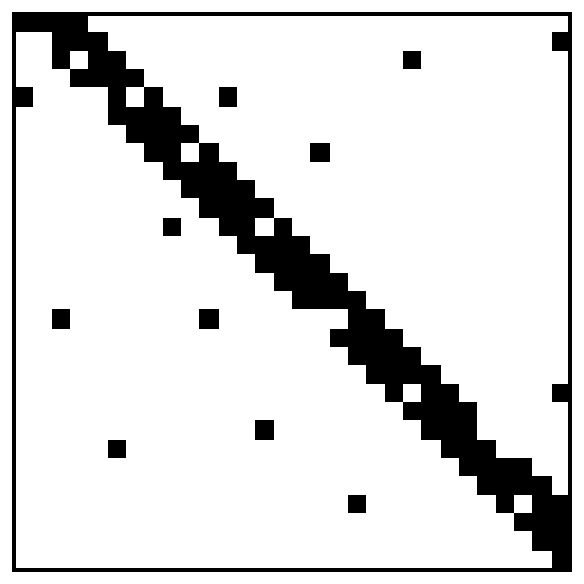
\includegraphics[width=.5\textwidth]{cqmat}
	\caption{C-diagonal Q-perturbed sparse matrix with Q=0.05 and C=4\label{fig:cqmat}}
\end{figure}

In this section, we introduced commonly used sparse matrix storage formats and the corresponding algorithm to perform the sparse matrix vector product as well as a way to parallelize the sparse matrix vector product and classical optimizations implemented in the sparse matrix vector product to improve its performances.
We also introduced C-diagonal Q-perturbed sparse matrices which are matrices that can be used as input to test the performances of the sparse matrix vector product.
In the last sections, we introduced the linear algebra methods we consider to implement to evaluate the task based programming models.
However, scientific applications cannot be reduced to only linear algebra methods so we also choose to study the Kirchhoff seismic pre-stack depth migration which will be introduced in the next section.

\section{Kirchhoff seismic pre-stack depth migration}

This section will present the Kirchhoff migration and continue the previous work made in \cite{rapport_Total_Petiton}.
This report explain the migration and gives hint to implement new algorithms for the migration.
This work take advantage from the discussions with Henri Calandra.
This section will detail the steps for the Kirchhoff migration.

\subsection{Overview}
The seismic migration is a technique used to visualize the underground.
Data are acquired at the surface during an acquisition campaign.
Data are processed to geometrically re-locate seismic events either in space or in time.
They are re-located to the location the event occurred in the subsurface rather than the location where it was recorded at the surface.
Migration moves dipping reflectors to their true subsurface positions and collapses diffractions, resulting in a migrated image that typically has an increased spatial resolution and resolves areas of complex geology much better than non-migrated images.
A form of migration is one of the standard data processing techniques for reflection-based geophysical methods (seismic reflection and ground-penetrating radar).

The Kirchhoff migration \cite{PingY1995} \cite{PTSCS2009} is a depth migration.
It is applied to seismic data in depth (regular Cartesian) coordinates, which must be calculated from seismic data in time coordinates.
This method does therefore require a velocity model, making it resource-intensive because building a seismic velocity model is a long and iterative process (Figure \ref{fig:kirchhoff-process}).
The significant advantage to this migration method is that it can be successfully used in areas with lateral velocity variations, which tend to be the areas that are most interesting to petroleum geologists.

\begin{figure}[H]
	\centering
	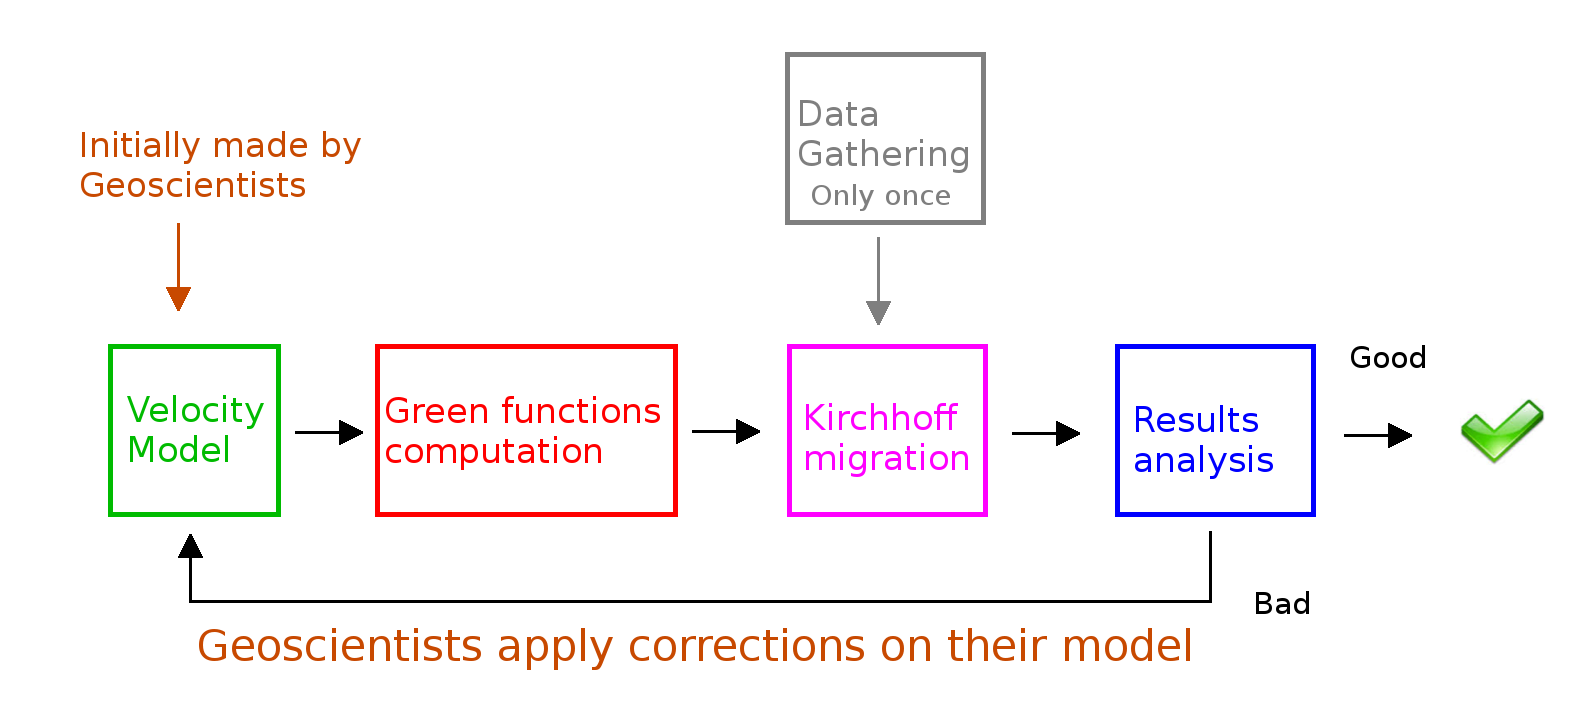
\includegraphics[scale=0.25]{kirchhoff-process}
	\caption{Building process of a seismic velocity model \label{fig:kirchhoff-process}}
\end{figure}

\subsection{Velocity model}
The velocity model describe the propagation speed of the waves into the different layer of the underground.
Geophysicists create a model and want to verify its correctness.
Their goal is to find the best model that explain the data.
They use the Kirchhoff migration that determine where are the limits between layers.
This method processes data called traces.
They are the output from a seismogram (receiver) at the surface after the emission (source) of a wave into the ground.
If the model is coherent with the image generated by the migration, the model is correct.
Otherwise, the model is adjusted by geophysicists and the migration is re-used to obtain a new image.
This process is repeated until the image and the model are coherent.

\subsection{Data gathering}
Data are produced during an acquisition campaign.
A campaign contains several shots.
A shot is a seismic impulsion launched through the ground.
It is the source (see Figure \ref{fig:shot}).
There is several receiver.
They are seismograms placed on a 2D grid on the ground (see Figure \ref{fig:source-receiver}).
The source is moved on the 2D grid and produces shots.
So a trace is the result for a given shot (source) and a given seismogram (receiver).

\begin{figure}[H]
	\centering
	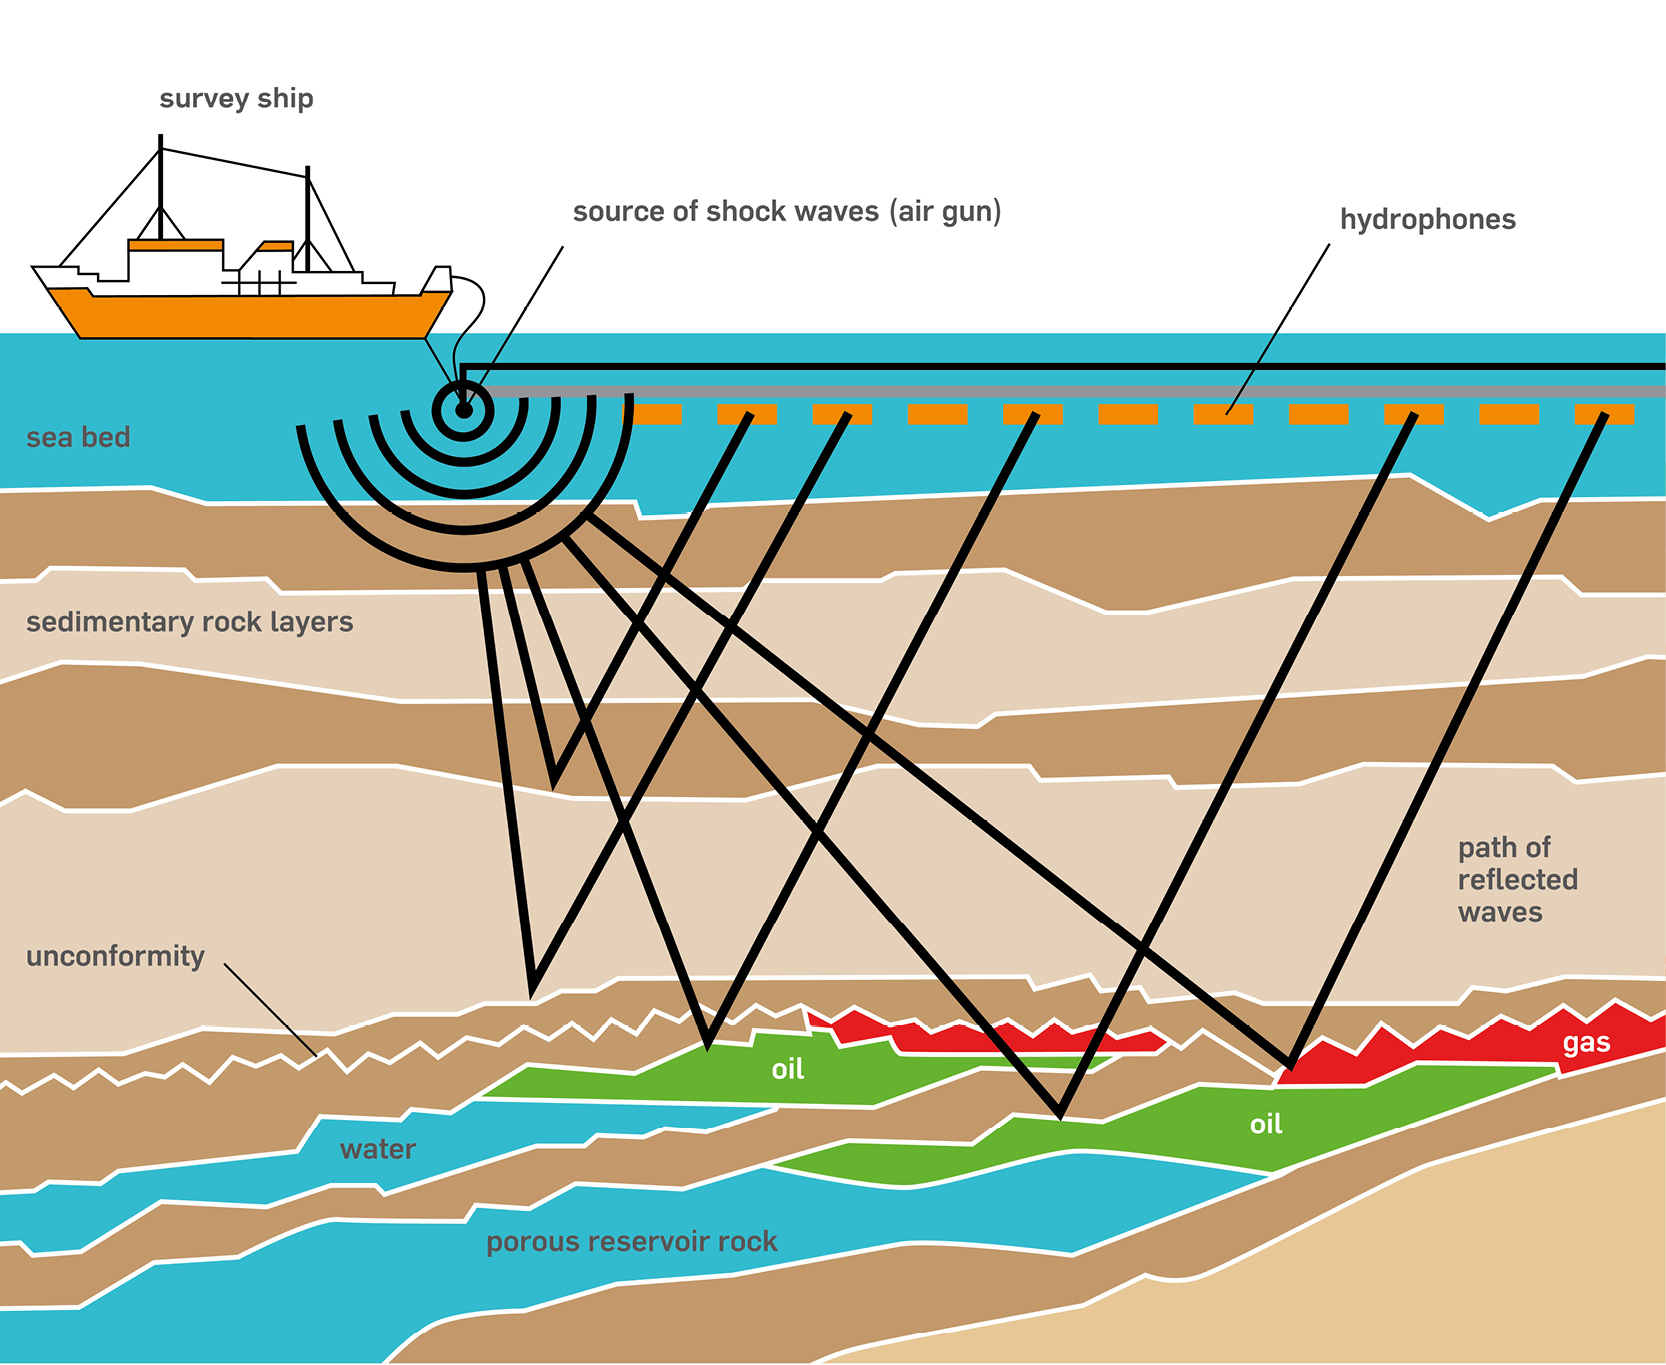
\includegraphics[scale=0.75]{oss}
	\caption{Shot during Data acquisition \label{fig:shot}}
\end{figure}
\begin{figure}[H]
	\centering
	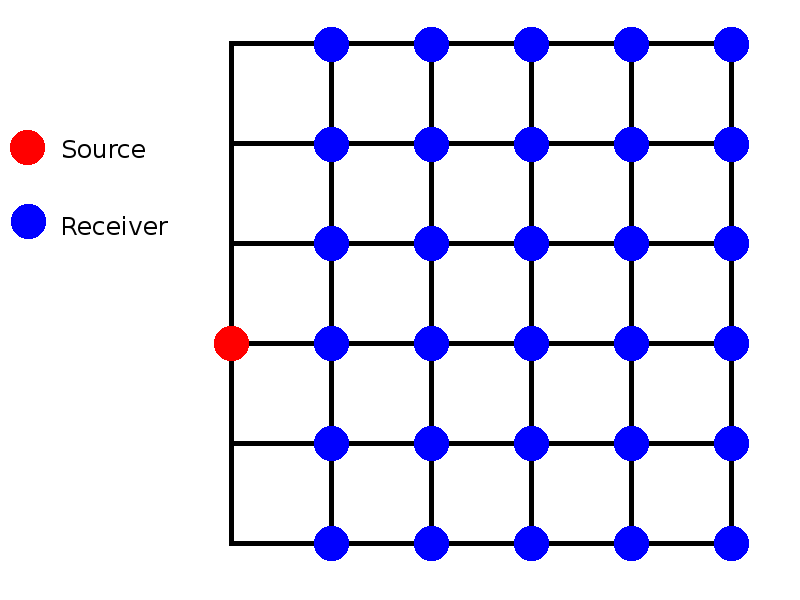
\includegraphics[scale=0.37]{gridSR}
	\caption{Shot and seismograms \label{fig:source-receiver}}
\end{figure}

The acquisition campaign gives a huge amount of traces since there is a lot of receiver and several shots.
A trace contains the coordinates of the source and the receiver and the data from the seismogram.

\subsection{Green functions}
The Green functions represent the response and the behaviour of the wave when the source is a Dirac impulse.
They allow to solve the wave equation using an integral formula in function of the source of the wave.
The behaviour of the wave in the ground depends on the velocity model.
Usually, Green functions are pre-calculated and stored on disk for a 2D grid on surface and a 3D grid underground.
During the building of the model and the migration, Green functions are retrieved from disk.

In the Kirchhoff migration, the Green functions are used to estimate the travel time between 2 points depending on the velocity model.
We estimate the travel time between a source S and a point P of the image ($T_{SP}$) then between P and a receiver R ($T_{PR}$).
So we can deduce $T_{SPR} = T_{SP} + T_{PR}$ (see Figure \ref{fig:Green_functions1}).

\begin{figure}[H]
	\centering
	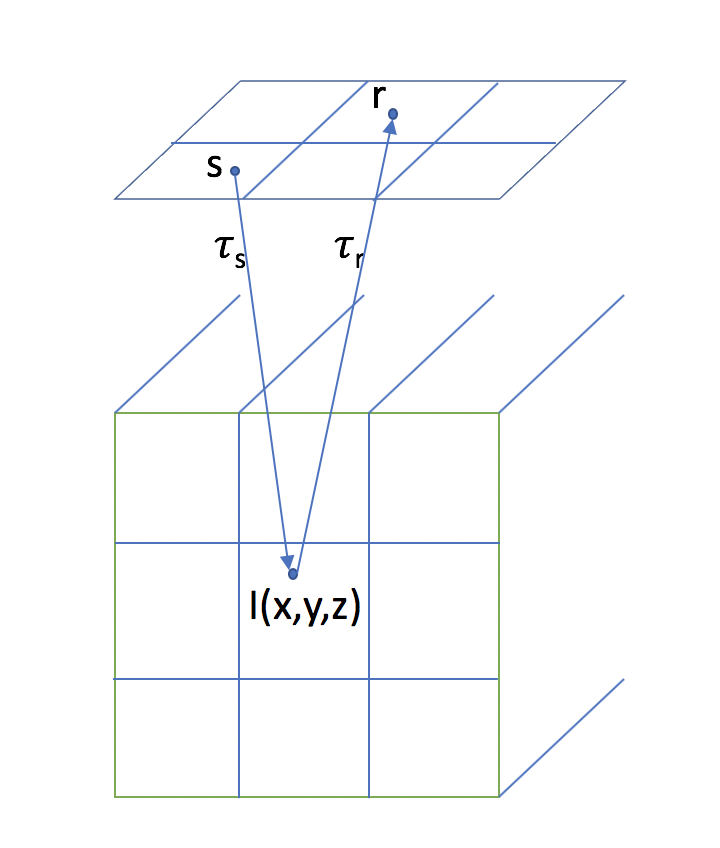
\includegraphics[scale=0.6]{img1}
	\caption{Wave travel between S and R through P\label{fig:Green_functions1} from \cite{rapport_Total_Petiton}}
\end{figure}

Green functions are pre-calculated for a 2D grid at the surface and for à 3D grid underground (see Figure \ref{fig:grids}).
Moreover, a block of the 3D grid contains an image at a finer grain.
Therefore, it is necessary to interpolate or extrapolate the Green functions for the points into the finer grid (see Figure \ref{fig:fine_coarse_grid}).

\begin{figure}[H]
	\centering
	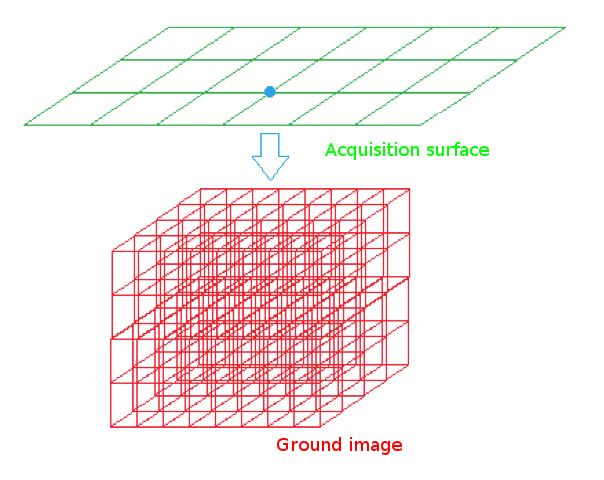
\includegraphics[width=.55\textwidth]{figure8rapportP2}
	\caption{2D and 3D grids \label{fig:grids} from \cite{rapport_Total_Petiton}}
\end{figure}

\begin{figure}[H]
	\centering
	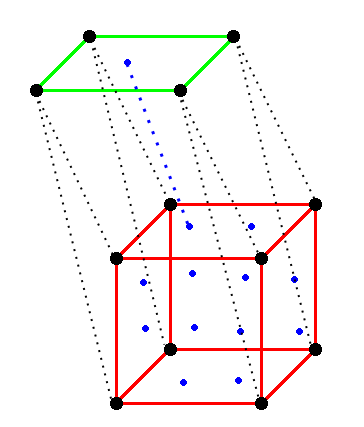
\includegraphics[width=.55\textwidth]{fctGreenInterpolation}
	\caption{Coarse grid and points from the finer grid \label{fig:fine_coarse_grid}}
\end{figure}

\subsection{Kirchhoff migration \label{sec:kirchhoff}}
The Kirchhoff migration produces a 3D image of the subsurface by retrieving the position of the reflection points in order to show the different layers of the ground.
To do so, find the time a wave need to travel from a source to a point $(x,y,z)$ in the image and travel back from this point to the receiver is necessary.
The Green functions in the fine grid give this time.
Then, the trace\footnote{http://www.iris.washington.edu/ds/nodes/dmc/manuals/irisfetchm/} (Figure \ref{fig:kir_trace}) has a peak when the wave arrives to the receiver.
This corresponds to the time it needs for the trace to travel from the source to the receiver into the ground.
For a given source and receiver, if the time a wave need to travel trough the point $(x,y,z)$ and the time to the peak of the trace match then $(x,y,z)$ can be a candidate to a reflection point.

\begin{figure}[H]
	\centering
	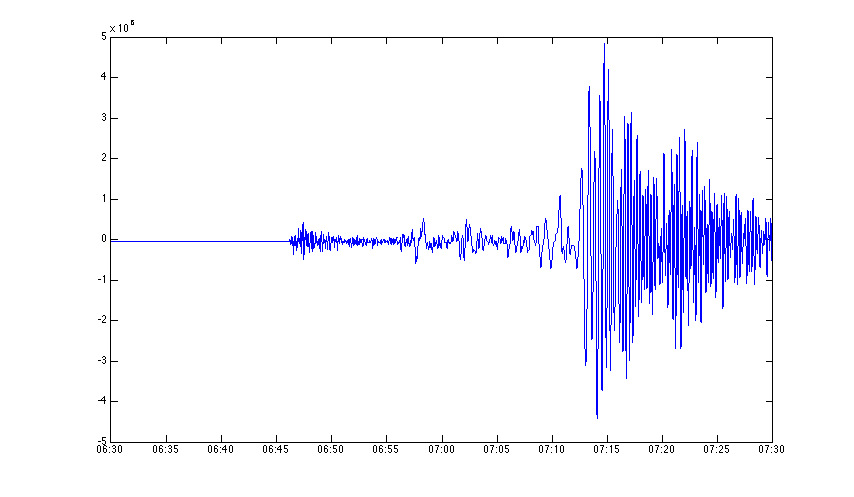
\includegraphics[width=.75\textwidth]{trace}
	%http://www.iris.washington.edu/ds/newsletter/vol14/no1/7/direct-data-access-from-within-matlab/
	\caption{A trace from the IRIS-DMC repository\label{fig:kir_trace}}
\end{figure}

Moreover, we know the Green functions for a coarse grain of the image, so it is possible to know if the points in the sub-domain of the coarse grid will match the time from the trace.
If the time matches, the points will be studied at a finer grain.
Otherwise, the points of the part of the coarse grid will not be candidates to a reflection point and those points will be ignored for the selected trace.

At the finer grain level, when the block of coarse grid matches with the time of the trace, the Green functions are interpolated or extrapolated for each point in the block.
This give the travel time $T(x,y,z)$ between the source and the receiver passing by the point $(x,y,z)$.
Then, only the points matching the time of the trace are kept.
Those points are likely true reflection points.
An arbitrary value (the aperture) $A_{s,r}(x,y,z)$  \cite{XHCCC2014} that favours points with less awkward reflection angles, and positions that are more likely to match the true reflection point, can be calculated.
This value depends on the coordinates of the receiver 'r', the coordinates of the source 's' and the point $(x,y,z)$.
The value $A_{s,r}(x,y,z) t_{s,r}(x,y,z)$ expresses the intensity of the contribution of the trace for the point $(x,y,z)$.

The image at a point is generated by summing the contribution of all the traces that can be a true reflection point :


\begin{equation}
	I(x,y,z)=\sum_{t_{s,r} \in T}A_{s,r}(x,y,z)t_{s,r}(\tau_s(x,y,z) + \tau_r(x,y,z))
\end{equation}

$I(x,y,z)$ is the point $(x,y,z)$ of the image.
$t_{s,r}$ is the trace which has $s$ as source and $r$ as receiver.
$T$ is the ensemble of traces.
$A_{s,r}$ is the amplitude associated to $s$ and $r$.
$\tau_j(x,y,z)$  is the time need for a wave to travel from $j$ (a source or a receiver) to $(x,y,z)$.


In the existing application, the Green functions (the time needed by the sound wave to go from the source or the receiver to the point inside the grid, the values of $\tau$) are pre-computed from the velocity model which is evaluated and imported from the file system when the application is using them.

Moreover, two granularities of grids are used.
The values of $A$ and $\tau$ are computed for the coarse grid and they are interpolated from the computed values for the fine grid.


\subsection{Analysis of the results}
The resulting image is analysed by geophysicists.
If they think that the velocity model is coherent with the image, the model can be exploited.
Otherwise, the velocity model is modified and the process of the Kirchhoff migration is reused until the geophysicists judge that the velocity model corresponds to the data.